\section{Experiments}
\label{sec:exp}

\paragraph{Protocol.} \Cref{tab:main} and every number in \cref{sec:main,sec:exp_gates,sec:exp_neg} come from one front-end pass over the 526 clips with the final system and its registered variants, read together with the original clips and \steer's outputs in one evaluation job (\cref{sec:metrics}). Every other table comes from its own pass and its own evaluation run; because the appearance distance is normalised within a run, it is compared only within a table. Paired differences carry 95\% bootstrap CIs over clips (10{,}000 resamples)~\cite{efron1994bootstrap} and readability differences exact McNemar tests~\cite{mcnemar1947}. \Cref{tab:main} reports all clips and, separately, the 486 clips never inspected during development. \textbf{Baseline.} \steer~\cite{zeng2026steervte}, the strongest published video text editor (glyph and style conditioning on a frozen VACE-14B backbone, one million training triplets), is run with the hint box as editing mask and the target as text at the input's resolution and length.

% generated by paper_numbers.py: Table 1 from r1full (one front-end pass, one evaluation job)
\begin{table*}[t]
\centering
\caption{\textbf{Main results} (526 clips; one front-end pass and one evaluation job for every row). Readability: share of clips whose text the reader transcribes exactly in at least 4 of 5 frames. Fixed / broken: garbled $\to$ correct and correct $\to$ wrong transitions relative to the original as read in the same job; net = fixed $-$ broken. Appearance: glyph-agnostic material distance to the original text (normalised within this run; lower is closer). BG PSNR: outside the dilated text region. Flicker and jitter: motion-compensated, inside the text box (grey levels). The lower block excludes the 40 clips inspected while developing the selective-editing components.}
\label{tab:main}
\setlength{\tabcolsep}{4.5pt}
\resizebox{\linewidth}{!}{%
\begin{tabular}{@{}lccccccccc@{}}
\toprule
 & Readability $\uparrow$ & Fixed $\uparrow$ & Broken $\downarrow$ & Net $\uparrow$ & NED sim.\ $\uparrow$ & Appearance $\downarrow$ & BG PSNR $\uparrow$ & Flicker $\downarrow$ & Jitter $\downarrow$ \\
\midrule
\multicolumn{10}{@{}l}{\emph{All 526 clips}} \\
Original (generated) & 53.8 & -- & -- & -- & 0.820 & -- & -- & 1.98 & 9.18 \\
\steer~\cite{zeng2026steervte} & 84.0 & 165 & \textbf{6} & 159 & 0.946 & \textbf{1.83} & 36.49 & \textbf{1.66} & 8.30 \\
\method & \textbf{91.4} & \textbf{210} & 12 & \textbf{198} & \textbf{0.959} & 2.57 & \textbf{42.52} & 1.79 & \textbf{7.86} \\
\midrule
\multicolumn{10}{@{}l}{\emph{486 clips outside the development set}} \\
Original (generated) & 54.7 & -- & -- & -- & 0.822 & -- & -- & 1.97 & 9.12 \\
\steer~\cite{zeng2026steervte} & 84.4 & 150 & \textbf{6} & 144 & 0.945 & \textbf{1.85} & 36.40 & \textbf{1.65} & 8.24 \\
\method & \textbf{91.2} & \textbf{189} & 12 & \textbf{177} & \textbf{0.958} & 2.60 & \textbf{42.50} & 1.79 & \textbf{7.86} \\
\bottomrule
\end{tabular}}
\end{table*}


\subsection{Main results}
\label{sec:main}
\method makes \rOursRead\% of the clips readable, \rReadGain{} points more than \steer (\rOnlyOurs{} clips correct only with \method, \rOnlySteer{} only with \steer; $p=\rMcNemarP$), and repairs \rOursFixed{} of the \rGarbled{} garbled clips. It breaks \rOursBroken{} of the \rOrigCorrect{} originally correct clips where \steer breaks \rSteerBroken, so its advantage in net repairs (\rOursNet{} vs.\ \rSteerNet) is smaller than in repairs alone; the picture is unchanged outside the development set (\rOursReadND\% vs.\ \rSteerReadND\%). The two methods trade different qualities: \method leaves the background intact (PSNR \rBGDiff\,dB higher, 95\% CI [\rBGDiffLo, \rBGDiffHi]) and its strokes jitter less (\rOursJitter{} vs.\ \rSteerJitter), because every glyph is placed once on the tracked carrier; \steer's region flickers less and, above all, its text looks more like the original (appearance distance \rSteerMad{} vs.\ \rOursMad), a gap we analyse in \cref{sec:limits}. \method is ahead on all seven materials, most on signboards (+\rGainSignboard{} points) and neon (+\rGainNeon), least on metal (+\rGainMetal) and wood (+\rGainWood), and reaches \rOursEn\% on English and \rOursZh\% on Chinese clips (\steer: \rSteerEn\%, \rSteerZh\%). \Cref{fig:qual} shows random examples, including two failures of \method.

\paragraph{A second reader.} Readability depends on the reader, so we registered a re-reading of the outputs by readers from other model families with identical crops, frames, prompt, decoding and scoring, and a rule fixed in advance: the advantage counts as reader-robust only if InternVL2.5-8B finds \method more readable than \steer with $p<0.05$. It does: \jIvlOurs\% against \jIvlSteer\% (\jIvlOnlyOurs{} vs.\ \jIvlOnlySteer{} discordant clips, $p=\jIvlP$), with a smaller margin that is significant for Chinese ($p=\jIvlZhP$) but not for English alone. A third reader, Pixtral-12B, cannot read Chinese and finds no advantage on the English clips (\jPixOurs\% vs.\ \jPixSteer\%); most of its errors on \method's outputs are correct transcriptions followed by invented text, which exact matching counts as wrong. Full tables are in the supplement, Sec.~B.

\paragraph{Edit locality.} \steer's difference to the original covers the entire frame, including edges far from the text; \method's is confined to the text region, with a residual of 1--2 grey levels elsewhere from re-encoding. Inside the text neighbourhood, the collateral change outside both old and new glyphs is \rOursCollat{} grey levels on the \rOursCollatN{} clips \method edits.

\begin{figure*}[t]
\centering
\setlength{\tabcolsep}{1.2pt}\renewcommand{\arraystretch}{0.6}
\begin{tabular}{@{}m{0.95cm}cccccc@{}}
&\footnotesize\textbf{Original} & \footnotesize\textbf{SteerVTE} & \footnotesize\textbf{Banksy} & \footnotesize\textbf{Original} & \footnotesize\textbf{SteerVTE} & \footnotesize\textbf{Banksy} \\[2pt]
\scriptsize neon & 
\includegraphics[width=0.146\linewidth]{figs/cells/qual_g001_en_neon_s2_orig.jpg} & 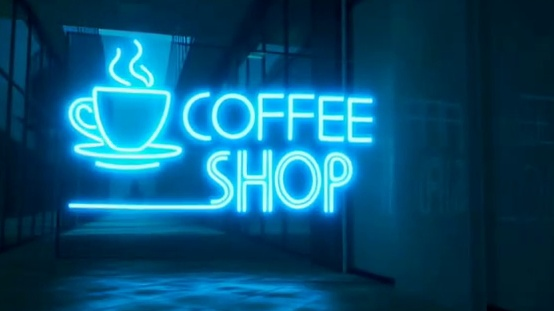
\includegraphics[width=0.146\linewidth]{figs/cells/qual_g001_en_neon_s2_steervte.jpg} & 
\includegraphics[width=0.146\linewidth]{figs/cells/qual_g001_en_neon_s2_B1.jpg} & 
\includegraphics[width=0.146\linewidth]{figs/cells/qual_g100_zh_neon_s5_orig.jpg} & 
\includegraphics[width=0.146\linewidth]{figs/cells/qual_g100_zh_neon_s5_steervte.jpg} & 
\includegraphics[width=0.146\linewidth]{figs/cells/qual_g100_zh_neon_s5_B1.jpg} \\
&\parbox[t]{0.146\linewidth}{\centering\scriptsize \textcolor{badred}{\ding{55}}\,\texttt{OFFEE SHOP}} & \parbox[t]{0.146\linewidth}{\centering\scriptsize \textcolor{okgreen}{\ding{51}}\,\texttt{COFFEE SHOP}} & \parbox[t]{0.146\linewidth}{\centering\scriptsize \textcolor{okgreen}{\ding{51}}\,\texttt{COFFEE SHOP}} & \parbox[t]{0.146\linewidth}{\centering\scriptsize \textcolor{badred}{\ding{55}}\,\texttt{\zh{公公}}} & \parbox[t]{0.146\linewidth}{\centering\scriptsize \textcolor{okgreen}{\ding{51}}\,\texttt{\zh{公园}}} & \parbox[t]{0.146\linewidth}{\centering\scriptsize \textcolor{badred}{\ding{55}}\,\texttt{\zh{公园}}} \\[3pt]
\scriptsize signboard & 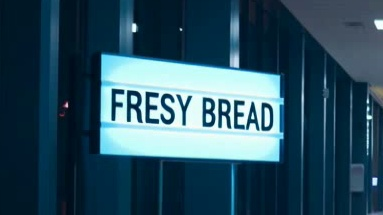
\includegraphics[width=0.146\linewidth]{figs/cells/qual_g008_en_signboard_s4_orig.jpg} & 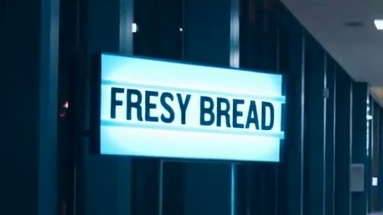
\includegraphics[width=0.146\linewidth]{figs/cells/qual_g008_en_signboard_s4_steervte.jpg} & 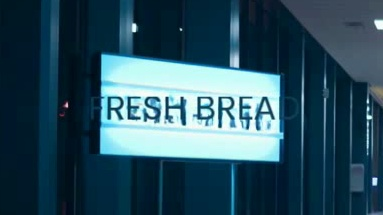
\includegraphics[width=0.146\linewidth]{figs/cells/qual_g008_en_signboard_s4_B1.jpg} & 
\includegraphics[width=0.146\linewidth]{figs/cells/qual_g085_zh_signboard_s8_orig.jpg} & 
\includegraphics[width=0.146\linewidth]{figs/cells/qual_g085_zh_signboard_s8_steervte.jpg} & 
\includegraphics[width=0.146\linewidth]{figs/cells/qual_g085_zh_signboard_s8_B1.jpg} \\
&\parbox[t]{0.146\linewidth}{\centering\scriptsize \textcolor{badred}{\ding{55}}\,\texttt{FRESY BREAD}} & \parbox[t]{0.146\linewidth}{\centering\scriptsize \textcolor{badred}{\ding{55}}\,\texttt{FRESY BREAD}} & \parbox[t]{0.146\linewidth}{\centering\scriptsize \textcolor{okgreen}{\ding{51}}\,\texttt{FRESH BREAD}} & \parbox[t]{0.146\linewidth}{\centering\scriptsize \textcolor{badred}{\ding{55}}\,\texttt{\zh{夜市} Qingdao Night Marke}} & \parbox[t]{0.146\linewidth}{\centering\scriptsize \textcolor{okgreen}{\ding{51}}\,\texttt{\zh{夜市}}} & \parbox[t]{0.146\linewidth}{\centering\scriptsize \textcolor{okgreen}{\ding{51}}\,\texttt{\zh{夜市}}} \\[3pt]
\scriptsize wood & 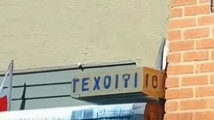
\includegraphics[width=0.146\linewidth]{figs/cells/qual_g014_en_wood_s6_orig.jpg} & 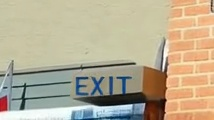
\includegraphics[width=0.146\linewidth]{figs/cells/qual_g014_en_wood_s6_steervte.jpg} & 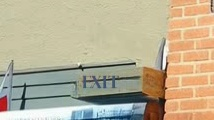
\includegraphics[width=0.146\linewidth]{figs/cells/qual_g014_en_wood_s6_B1.jpg} & 
\includegraphics[width=0.146\linewidth]{figs/cells/qual_g105_zh_wood_s1_orig.jpg} & 
\includegraphics[width=0.146\linewidth]{figs/cells/qual_g105_zh_wood_s1_steervte.jpg} & 
\includegraphics[width=0.146\linewidth]{figs/cells/qual_g105_zh_wood_s1_B1.jpg} \\
&\parbox[t]{0.146\linewidth}{\centering\scriptsize \textcolor{badred}{\ding{55}}\,\texttt{TEXOITYIO}} & \parbox[t]{0.146\linewidth}{\centering\scriptsize \textcolor{okgreen}{\ding{51}}\,\texttt{EXIT}} & \parbox[t]{0.146\linewidth}{\centering\scriptsize \textcolor{okgreen}{\ding{51}}\,\texttt{EXIT}} & \parbox[t]{0.146\linewidth}{\centering\scriptsize \textcolor{badred}{\ding{55}}\,\texttt{\zh{小悒念滑}}} & \parbox[t]{0.146\linewidth}{\centering\scriptsize \textcolor{okgreen}{\ding{51}}\,\texttt{\zh{小心地滑}}} & \parbox[t]{0.146\linewidth}{\centering\scriptsize \textcolor{okgreen}{\ding{51}}\,\texttt{\zh{小心地滑}}} \\[3pt]
\scriptsize metal & 
\includegraphics[width=0.146\linewidth]{figs/cells/qual_g024_en_metal_s2_orig.jpg} & 
\includegraphics[width=0.146\linewidth]{figs/cells/qual_g024_en_metal_s2_steervte.jpg} & 
\includegraphics[width=0.146\linewidth]{figs/cells/qual_g024_en_metal_s2_B1.jpg} & 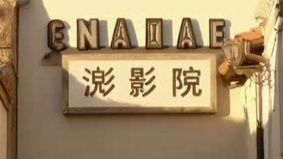
\includegraphics[width=0.146\linewidth]{figs/cells/qual_g089_zh_metal_s3_orig.jpg} & 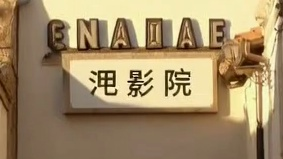
\includegraphics[width=0.146\linewidth]{figs/cells/qual_g089_zh_metal_s3_steervte.jpg} & 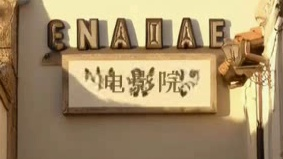
\includegraphics[width=0.146\linewidth]{figs/cells/qual_g089_zh_metal_s3_B1.jpg} \\
&\parbox[t]{0.146\linewidth}{\centering\scriptsize \textcolor{badred}{\ding{55}}\,\texttt{PHARMAICE}} & \parbox[t]{0.146\linewidth}{\centering\scriptsize \textcolor{okgreen}{\ding{51}}\,\texttt{PHARMACY}} & \parbox[t]{0.146\linewidth}{\centering\scriptsize \textcolor{okgreen}{\ding{51}}\,\texttt{PHARMACY}} & \parbox[t]{0.146\linewidth}{\centering\scriptsize \textcolor{badred}{\ding{55}}\,\texttt{\zh{澎影院}}} & \parbox[t]{0.146\linewidth}{\centering\scriptsize \textcolor{badred}{\ding{55}}\,\texttt{\zh{洹影院}}} & \parbox[t]{0.146\linewidth}{\centering\scriptsize \textcolor{okgreen}{\ding{51}}\,\texttt{\zh{电影院}}} \\[3pt]
\scriptsize glass & 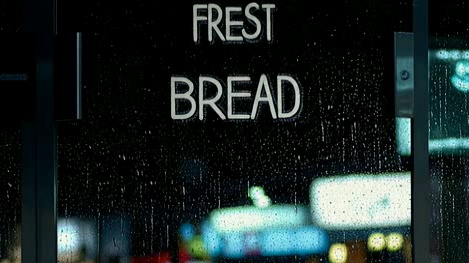
\includegraphics[width=0.146\linewidth]{figs/cells/qual_g007_en_glass_s2_orig.jpg} & 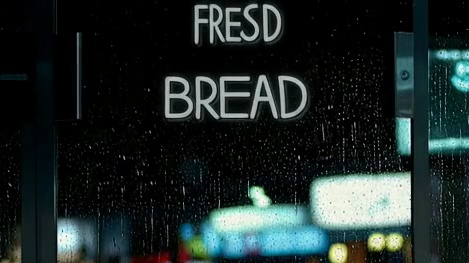
\includegraphics[width=0.146\linewidth]{figs/cells/qual_g007_en_glass_s2_steervte.jpg} & 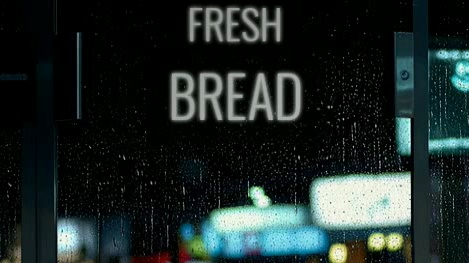
\includegraphics[width=0.146\linewidth]{figs/cells/qual_g007_en_glass_s2_B1.jpg} & 
\includegraphics[width=0.146\linewidth]{figs/cells/qual_g090_zh_glass_s7_orig.jpg} & 
\includegraphics[width=0.146\linewidth]{figs/cells/qual_g090_zh_glass_s7_steervte.jpg} & 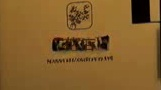
\includegraphics[width=0.146\linewidth]{figs/cells/qual_g090_zh_glass_s7_B1.jpg} \\
&\parbox[t]{0.146\linewidth}{\centering\scriptsize \textcolor{badred}{\ding{55}}\,\texttt{FREST BREAD}} & \parbox[t]{0.146\linewidth}{\centering\scriptsize \textcolor{badred}{\ding{55}}\,\texttt{FRESB BREAD}} & \parbox[t]{0.146\linewidth}{\centering\scriptsize \textcolor{okgreen}{\ding{51}}\,\texttt{FRESH BREAD}} & \parbox[t]{0.146\linewidth}{\centering\scriptsize \textcolor{badred}{\ding{55}}\,\texttt{\cjkimg{cjk_b7d9d7d024} HUAJANGDIAN}} & \parbox[t]{0.146\linewidth}{\centering\scriptsize \textcolor{okgreen}{\ding{51}}\,\texttt{\zh{花店}}} & \parbox[t]{0.146\linewidth}{\centering\scriptsize \textcolor{badred}{\ding{55}}\,\texttt{\zh{南湖公园}}} \\[3pt]
\scriptsize paper & 
\includegraphics[width=0.146\linewidth]{figs/cells/qual_g034_en_paper_s3_orig.jpg} & 
\includegraphics[width=0.146\linewidth]{figs/cells/qual_g034_en_paper_s3_steervte.jpg} & 
\includegraphics[width=0.146\linewidth]{figs/cells/qual_g034_en_paper_s3_B1.jpg} & 
\includegraphics[width=0.146\linewidth]{figs/cells/qual_g096_zh_paper_s0_orig.jpg} & 
\includegraphics[width=0.146\linewidth]{figs/cells/qual_g096_zh_paper_s0_steervte.jpg} & 
\includegraphics[width=0.146\linewidth]{figs/cells/qual_g096_zh_paper_s0_B1.jpg} \\
&\parbox[t]{0.146\linewidth}{\centering\scriptsize \textcolor{badred}{\ding{55}}\,\texttt{SALE}} & \parbox[t]{0.146\linewidth}{\centering\scriptsize \textcolor{badred}{\ding{55}}\,\texttt{SALE}} & \parbox[t]{0.146\linewidth}{\centering\scriptsize \textcolor{okgreen}{\ding{51}}\,\texttt{SALE 50\%}} & \parbox[t]{0.146\linewidth}{\centering\scriptsize \textcolor{badred}{\ding{55}}\,\texttt{\zh{洗衣}}} & \parbox[t]{0.146\linewidth}{\centering\scriptsize \textcolor{okgreen}{\ding{51}}\,\texttt{\zh{洗衣店}}} & \parbox[t]{0.146\linewidth}{\centering\scriptsize \textcolor{okgreen}{\ding{51}}\,\texttt{\zh{洗衣店}}} \\[3pt]
\scriptsize screen & 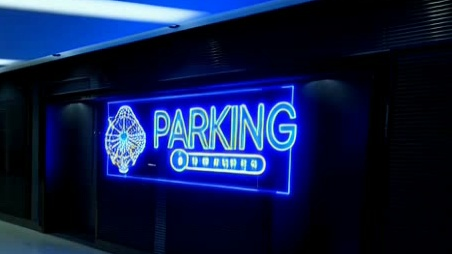
\includegraphics[width=0.146\linewidth]{figs/cells/qual_g029_en_screen_s3_orig.jpg} & 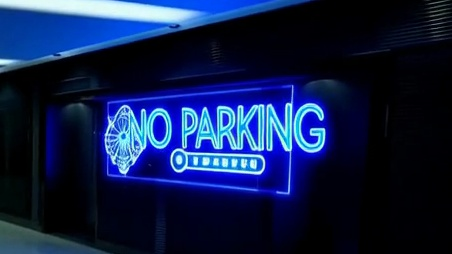
\includegraphics[width=0.146\linewidth]{figs/cells/qual_g029_en_screen_s3_steervte.jpg} & 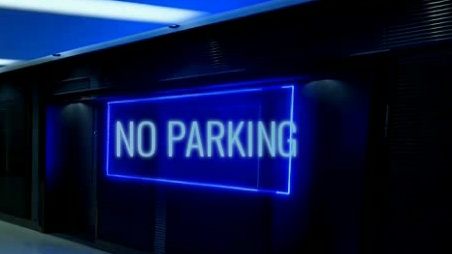
\includegraphics[width=0.146\linewidth]{figs/cells/qual_g029_en_screen_s3_B1.jpg} & 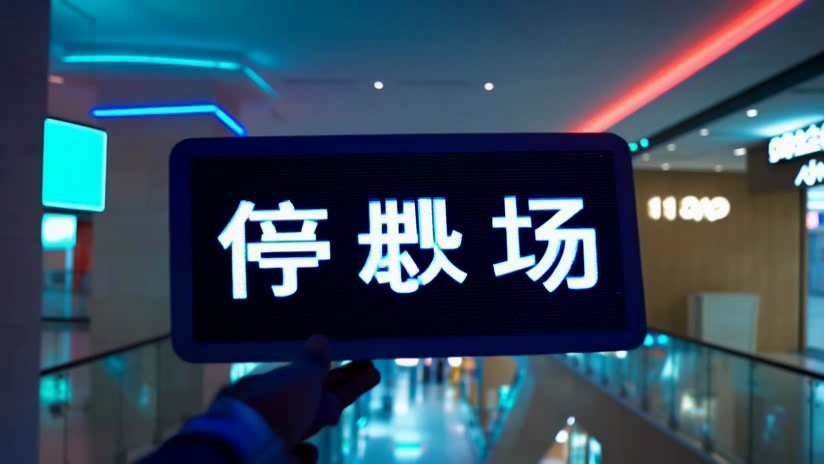
\includegraphics[width=0.146\linewidth]{figs/cells/qual_g078_zh_screen_s4_orig.jpg} & 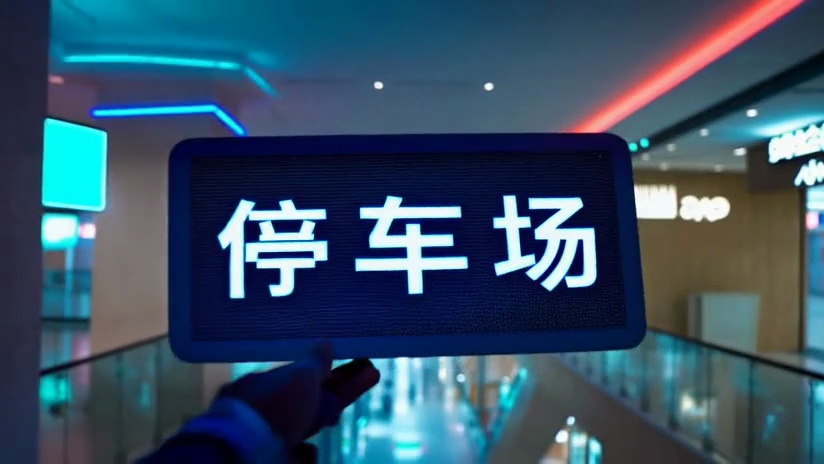
\includegraphics[width=0.146\linewidth]{figs/cells/qual_g078_zh_screen_s4_steervte.jpg} & 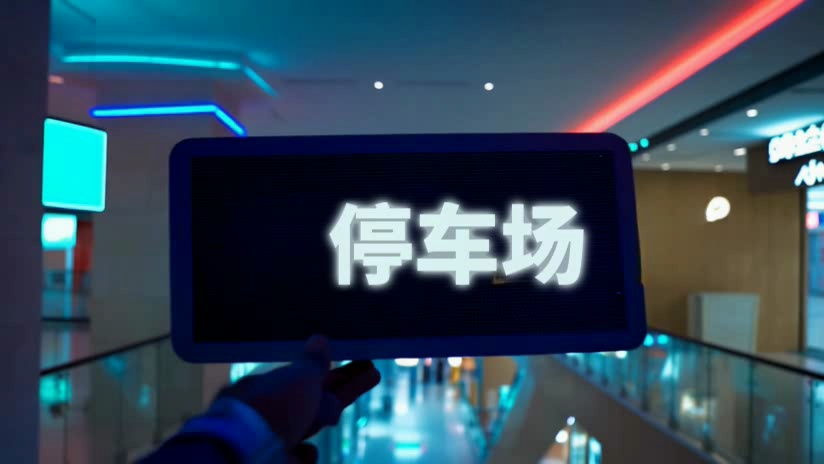
\includegraphics[width=0.146\linewidth]{figs/cells/qual_g078_zh_screen_s4_B1.jpg} \\
&\parbox[t]{0.146\linewidth}{\centering\scriptsize \textcolor{badred}{\ding{55}}\,\texttt{PARKING}} & \parbox[t]{0.146\linewidth}{\centering\scriptsize \textcolor{okgreen}{\ding{51}}\,\texttt{NO PARKING}} & \parbox[t]{0.146\linewidth}{\centering\scriptsize \textcolor{okgreen}{\ding{51}}\,\texttt{NO PARKING}} & \parbox[t]{0.146\linewidth}{\centering\scriptsize \textcolor{badred}{\ding{55}}\,\texttt{\cjkimg{cjk_9107d7aedf}}} & \parbox[t]{0.146\linewidth}{\centering\scriptsize \textcolor{okgreen}{\ding{51}}\,\texttt{\zh{停车场}}} & \parbox[t]{0.146\linewidth}{\centering\scriptsize \textcolor{okgreen}{\ding{51}}\,\texttt{\zh{停车场}}} \\[3pt]
\end{tabular}
\caption{\textbf{Qualitative comparison on randomly sampled clips} (one English and one Chinese clip per material, drawn with a fixed seed among garbled originals outside the development set; not curated). Each cell is the same crop of frame 24; below it, the reader's transcription (\textcolor{okgreen}{\ding{51}}~correct, \textcolor{badred}{\ding{55}}~wrong). SteerVTE produces more natural glyphs but frequently keeps or invents wrong characters; Banksy writes the target but its glyphs often look pasted (see \cref{sec:limits}).}
\label{fig:qual}
\end{figure*}


\subsection{The evidence gates}
\label{sec:exp_gates}
\paragraph{Preservation gate.} The gate skips \rSkipped{} clips, all confirmed correct by the reader (no false skip; the registered limit was 2\%). In the selective-editing pass (\cref{sec:exp_sel}) it is the only difference between B0 and B1: it restores \sRestored{} of the \sBrokenBzero{} originally correct clips that B0 breaks and loses none. Its recall is low by design: the pipeline's OCR rarely reads stylised originals---neon italics, extruded or condensed letters---consistently enough, and all \rOursBroken{} clips \method breaks are such cases (\cref{sec:failures}).

\paragraph{Carrier anchoring, font matching, localization gate.} Pasting the target into the per-frame OCR box makes the text readable but nearly doubles flicker (3.12 vs.\ 1.98 for the original), because OCR boxes jitter; anchoring everything on the tracked carrier brings it to the level of \steer (1.67 vs.\ 1.66) with lower jitter (7.12 vs.\ 8.30) and unchanged readability. Matching the font to the old strokes adds 2.6 points of readability ($p=0.044$) once candidates are rendered in the layout of the original. Laying the text out on the glyph instance leaves half as much of the old ink visible as the box layout (residual 0.21 vs.\ 0.42) but, with a confidence-based tracker, cost 5.5 points of readability; carrier tracking recovers most of it, and the localization gate routes the unreliable instances to the box layout, giving a front end as readable as the box layout (91.1 vs.\ 90.7) with the instance path's lower residual and lowest jitter. Two re-readings of the same outputs differ by about one point, so we claim parity, not superiority (supplement, Sec.~B).

\subsection{Source appearance transport}
\label{sec:exp_sat}
The appearance gate enables SAT on 53 clips of the analysed pass (23 neon, 11 screen, 9 signboard, 8 metal, 2 wood); most rejections are clips without an accepted instance, non-emissive text, or no cross-validated gain. On the enabled clips SAT reduces the appearance distance by a third ($-1.02$; better on 42 of 53 clips) for every material---screens 3.02$\to$1.33, neon 3.03$\to$2.02, wood 4.12$\to$2.21---without hurting readability or the background, at a cost in temporal stability (flicker $+0.15$, jitter $+0.81$). Because the distance is only a proxy, we ran a blind study on all 53 clips: raters saw the original between the paste-only and the SAT version in random order and answered three separate questions. With four raters (one excluded by a rule fixed after seeing the data; results with all five are reported too), SAT was judged closer to the original material in 158 of 182 non-tied judgements (win rate 0.87, 95\% CI [0.77, 0.94]; 48 vs.\ 3 clips by majority) and as having fewer artifacts in 147 of 191 (0.77 [0.66, 0.87]). The measured flicker increase was not perceived. The six clips raters judged worse show a bright rectangular plate behind the new letters, which we traced to the canvas truncating the halo's distance field; the fix was diagnosed on these clips and is therefore not part of the evaluated system (supplement, Sec.~B and F).

\subsection{Selective, structure-preserving editing}
\label{sec:exp_sel}
The most frequent problem of an early \method was not missing material but changing things it should not have. We therefore tested, with criteria fixed before the run, three components added to B0 (\method without the preservation gate): the preservation gate (B1), glyph-only erasure (B2) and a carrier-fit check that declares a target layout-infeasible (B3). In one front-end pass and one evaluation run, the preservation gate meets its criteria (no false skip, two fewer broken clips, readability not lower) and is adopted, which makes B1 the \method of \cref{tab:main}. Glyph-only erasure reduces collateral change on all clips ($\sBtwoCollatAll$, 95\% CI $[\sBtwoCollatAllLo, \sBtwoCollatAllHi]$) but not significantly outside the development clips, and costs \sBtwoCost{} points of readability because the instance ink mask is not a complete glyph mask; of 24 clips flagged infeasible, inspection confirmed 5. B2 and B3 are rejected (supplement, Sec.~B).

\subsection{What did not pass}
\label{sec:exp_neg}
We report the alternatives we built and rejected; each was judged by criteria fixed before its run, and all details are in the supplement, Sec.~C and D.

\paragraph{A learned refiner.} A video diffusion transformer initialised from Wan2.1-T2V-1.3B~\cite{wan2025wan}, trained as a flow-matching bridge~\cite{lipman2023flowmatching,liu2023rectifiedflow} from the pasted clip to the target on Blender renders, 562 real pairs and up to 1.15 million image pairs, does not improve on the paste it starts from: refiners trained with 0, 10k, 100k and 1M image pairs reach 75--78\% readability on a garbled subset against 80.7\% for the paste, and a diagnostic on 1{,}500 held-out pairs shows that they move away from the original even on the task they were trained for, because the paste's font and the generator's glyphs make the supervision inconsistent. Glyph-consistent supervision recovers most of the image-domain loss but still does not exceed the paste on video. On the full benchmark the best refiner costs 3.5 points of readability, adds flicker, jitter and chunk seams, and leaves the appearance distance unchanged ($-0.035$, 95\% CI $[-0.21, 0.19]$). The result is specific to our scale (1.3B parameters, a few hundred real video pairs), but at this scale a learned harmoniser trades the guarantee that motivates rendering for a gain we could not measure.

\paragraph{Two appearance modules.} Baseline-aligned layout with glyph-matched fonts (B1f) changes the output in \rTiltN{} and \rFshapeN{} clips respectively and leaves readability unchanged, but its appearance difference ($\rBOnefMadDiffND$ [$\rBOnefMadLoND$, $\rBOnefMadHiND$]) fails the registered criterion; the appearance distance is glyph-agnostic, so it cannot see what B1f changes, and we report the criterion unchanged rather than amend it. Reuse of the correctly generated source glyphs (R1), which keeps the right letters in place with their own material and renders only the missing ones, applies to only \rReuseApplied{} of the 526 clips with our current segmentation, matching and gating, too few to evaluate. Neither module is part of \method.

\paragraph{A glyph-locked material generator.} A conditional U-Net in the carrier's UV space, trained on 2{,}000 Blender counterfactual pairs that differ only in the text, closes 0.48 of the gap between a flat paste and the rendered truth on held-out pairs (registered gate 0.50; a model with 1.8$\times$ the parameters, the one registered capacity test, closes 0.498). Applied zero-shot to 129 benchmark clips it fails every registered criterion (appearance distance 3.06 vs.\ 1.99 for \method; 20 readings lost). Under our registered protocol, increasing capacity did not close the synthetic-domain criterion and zero-shot transfer to generated video degraded both appearance and readability; a photometric ablation attributes part of the transfer loss to the renders' photometry and leaves the rest unexplained by it.

\paragraph{Reconstruction without source glyphs.} \method's gating assumes that some glyph survives. Classifying the benchmark with the frozen localiser, \lthreeGlyphs{} clips have readable matches, \lthreeLtwo{} have detectable but unreadable pseudo-text (which \method handles through its detection-box fallback at \lthreeLtwoBoneRead\% readability; \steer: \lthreeLtwoSteerRead\%), and none lacks a detectable text-like region. To test the case the benchmark does not contain, we registered a branch that lays the target out from the tracked carrier alone and evaluated it on the \lthreeGlyphs{} clips with their glyphs erased: it reads \lthreeACarRead\% of the locatable clips where the frozen code's static-hint fallback reads \lthreeABfbRead\% and the deployed configuration writes nothing, but it misses the registered geometry and stability criteria (\lthreeAPassed{} of \lthreeACriteria), so the registered verdict is a failure. On the \lthreeLtwo{} natural pseudo-text clips, an amendment registered after the classes were known reads \lthreeBCarRead\% against \method's \lthreeBBoneRead\% ($p=\lthreeBP$) with no clip broken, but the appearance distance rises from \lthreeBBoneMad{} to \lthreeBCarMad; routing these clips to the branch would raise readability on the benchmark by about one point at that cost. The branch shows a readability gain on inputs that defeat the deployed system; it has not shown that it keeps the material and the stability of \method, and it is not part of \method.

\subsection{Verified selection between \method and \steer}
\label{sec:exp_hybrid}
% compact version of tables/tab_hybrid.tex for the 8-page main paper (same run, same numbers); the full table is in the supplement
\begin{table}[t]
\centering\small
\caption{\textbf{Verified selection between \method and \steer} (526 clips, one evaluation run; the full table with ablations is in the supplement, Sec.~B). Banksy-V keeps the clip when the preservation gate fires, otherwise takes a \steer output whose text an independent verifier (InternVL2.5-8B) reads as the target, composited locally into the original, and falls back to \method. W/L: clips correct only with the system / only with \method.}
\label{tab:hybrid}
\setlength{\tabcolsep}{3pt}
\resizebox{\linewidth}{!}{%
\begin{tabular}{@{}lcccccc@{}}
\toprule
 & Read.\ $\uparrow$ & Broken $\downarrow$ & Net $\uparrow$ & W/L & Appear.\ $\downarrow$ & BG PSNR $\uparrow$ \\
\midrule
\method (B1) & 91.8 & 12 & 201 & -- & 3.34 & 42.52 \\
\steer & 84.0 & 5 & 160 & 29/70 & 2.37 & 36.49 \\
Banksy-V (verified, local) & 96.4 & 0 & 225 & 30/6 & 2.67 & 41.74 \\
Oracle selection (upper bound) & 98.1 & 0 & 234 & 34/1 & 2.70 & 41.74 \\
\bottomrule
\end{tabular}}
\end{table}

The two systems fail on different clips, so a system that could tell which output is right would inherit the readability of both. We registered one before running it, with no tunable threshold: \emph{Banksy-V} keeps the clip when the preservation gate fires; otherwise it runs \steer (seed 1, then a second seed) and accepts an output whose text an independent verifier---InternVL2.5-8B with the reading protocol of \cref{sec:metrics}---transcribes as the target in at least 4 of 5 frames, composited back into the original around the text box with a feathered boundary and a colour match; otherwise it falls back to \method. The verifier never scores. In one run over every row (\cref{tab:hybrid}), Banksy-V reads correctly in \hVRead\% of the clips (\hVOnlySys{} vs.\ \hVOnlyBone{} discordant against \method, $p=\hVP$) with \hVBroken{} broken clips and \hVNet{} net repairs; its appearance distance lies between \steer's and \method's, because \steer's text is used wherever it reads correctly, and the background stays local (\hVBG\,dB). It meets five of six registered criteria and misses the temporal one by a margin that we trace to the re-encoding of the composited output (supplement, Sec.~B). Banksy-V is a system combination---its material from \steer, its correctness from verification, its locality and fallback from \method---and it runs \steer up to twice per clip plus a 7B verifier; a registered blind study of its naturalness against \steer is in progress and is not reported here.

\subsection{External benchmarks}
\label{sec:exp_external}
On \steer's own VTE-Bench Real (100 real clips whose correct text is to be changed), the frozen \method is clearly behind \steer (\xVteOurs\% vs.\ \xVteSteer\%), partly because its front end does not locate \xVteFails{} of the source texts and ships those clips unchanged: on correct, well-formed text the gates that make \method safe for repair have nothing to protect. On the 29 replacement and translation clips of VidScribe~\cite{vidscribe2026} that OCR can locate, \method reads \xVsOurs\%, ahead of the strongest of seven commercial models (\xVsBest\%) without significance and significantly ahead of \xVsSig{} of them, with the background kept (\xVsOursBG\,dB against \xVsBGLo--\xVsBGHi\,dB). We report both to delimit the claim: \method is a repair method for garbled generated text, not a general video text editor (supplement, Sec.~B).
